\documentclass[10pt,twocolumn]{article}

\usepackage[margin=0.72in,columnsep=0.28in]{geometry}
\usepackage{mathptmx}
\usepackage{amsmath,amssymb}
\usepackage{graphicx}
\usepackage{booktabs}
\usepackage{caption}
\usepackage[hidelinks]{hyperref}
\usepackage{titlesec}
\usepackage{threeparttable}

\titlespacing*{\section}{0pt}{8pt}{4pt}
\titlespacing*{\subsection}{0pt}{6pt}{3pt}
\setlength{\abovecaptionskip}{4pt}
\setlength{\belowcaptionskip}{-4pt}

\title{\vspace{-1.5em}\Large A Harmonic-Comb Parametric Estimator for the Cyclic Spectral Alpha Profile\vspace{-0.5em}}
\author{}
\date{}

\begin{document}
\twocolumn[
  \begin{@twocolumnfalse}
    \maketitle
    \vspace{-2.8em}
    \begin{center}
    \begin{minipage}{0.92\textwidth}
    \small
    \textbf{Abstract}\,---\,
    The spectral correlation density (SCD) of a cyclostationary signal is
    routinely summarized by its \emph{alpha profile}, the maximum of the
    SCD magnitude over spectral frequency at each cycle frequency. Sparse
    reconstruction methods for the strip spectral correlation analyzer
    (SSCA) accelerate SCD estimation by exploiting sparsity in the cycle
    frequency domain, but their accuracy degrades when the underlying
    cyclic spectrum is only approximately sparse, as is the case for
    direct-sequence spread-spectrum modulation. It is shown here that the
    alpha profile itself is a substantially sparser object than the full
    SCD surface: for a signal with a single fundamental cycle frequency
    $\alpha_0$, the profile's support is confined to the harmonic comb
    $\{m\alpha_0\}$. A parametric estimator is derived that recovers this
    comb directly from the signal's cyclic autocorrelation, evaluated on a
    subsampled index set at a small number of lags. The fundamental
    frequency is located by a combined-lag detection statistic and refined
    with a harmonic-consistency rule that resolves sub- and super-harmonic
    ambiguity. It is further shown that the statistic, although evaluated
    from few samples, can be computed exactly at every native frequency
    bin by a single zero-padded fast Fourier transform per lag, rather
    than by direct summation over a resolution-matched search grid,
    reducing the dominant computational cost from one that grows with the
    product of sample count and grid size to one that is independent of
    sample count. On a direct-sequence spread-spectrum binary phase-shift
    keyed test signal, the resulting estimator recovers the alpha profile
    from a few percent of the available samples and executes faster than
    both dense and sparse SCD reconstruction, at the cost of higher
    profile-magnitude error relative to full reconstruction.
    \end{minipage}
    \end{center}
    \vspace{1.2em}
  \end{@twocolumnfalse}
]

\section{Introduction}

A signal $x(t)$ is second-order cyclostationary if its autocorrelation is
periodic in time rather than constant, a property exhibited by essentially
all digitally modulated communication signals. The spectral correlation
density (SCD) $S_X^{\alpha}(f)$ generalizes the power spectral density to
this setting, indexed jointly by spectral frequency $f$ and \emph{cycle
frequency} $\alpha$ \cite{gardner1986}. For a linearly modulated signal the
SCD is concentrated at a discrete set of cycle frequencies determined by
the symbol or chip rate, which is what makes cyclostationary analysis a
standard tool for signal detection and classification.

The strip spectral correlation analyzer (SSCA) is the conventional
algorithm for estimating $S_X^{\alpha}(f)$ from data
\cite{roberts1991}. It channelizes the input, forms a channel-data product
by multiplying each channel's complex demodulate against the conjugated
input, and applies a further Fourier transform along time to resolve
$\alpha$. This last transform dominates the cost of the algorithm, since it
is applied once per channel over the full record length. Because the
resulting cyclic spectrum is sparse in $\alpha$ for most signals of
interest, this transform has been replaced with sparse Fourier
transform algorithms, giving a sparse SSCA (S3CA) with substantially
reduced sample and computational requirements \cite{s3ca2015,
hassanieh2012}.

Sparse reconstruction of this kind assumes that the cyclic spectrum is
close to exactly $\kappa$-sparse: that all but a bounded number of
coefficients are negligible. This assumption is well matched to a clean
tone or narrowband carrier, but is violated by direct-sequence
spread-spectrum (DSSS) signals, whose pseudo-random chip sequence spreads
energy broadly across the spectrum in addition to the narrow cyclic
features associated with the underlying symbol rate. The resulting cyclic
spectrum is only \emph{approximately} sparse: a bounded set of coefficients
captures the great majority, but not all, of its energy.

This paper considers a different summary of the SCD, the \emph{alpha
profile}
\begin{equation}
P(\alpha) = \max_{f} \left| S_X^{\alpha}(f) \right|,
\label{eq:profile}
\end{equation}
which reports cyclic feature strength independently of spectral location
and is the quantity most commonly consulted for detection and
classification. It is shown that, unlike the full SCD surface, the alpha
profile of a signal with a single fundamental cycle frequency is supported
almost entirely on the harmonic comb $\{m\alpha_0 : m \in \mathbb{Z}\}$,
and is therefore genuinely sparse even when the underlying SCD is not.
This motivates a parametric estimator that recovers the profile directly
from a small subsample of the signal, bypassing SCD reconstruction
entirely. The remainder of the paper derives this estimator, analyzes its
computational cost relative to dense and sparse SCD reconstruction, and
reports its accuracy on a DSSS binary phase-shift-keyed (BPSK) test signal.

\section{Signal Model and Problem Formulation}

The channelized complex demodulate at channel center frequency
$f_k = k/N_P$, $k \in \{-\lfloor N_P/2 \rfloor, \dots\}$, is formed as
\begin{equation}
X_T(t,f_k) = \left[ \sum_{r} a(r)\, x(t+r)\, e^{-i2\pi f_k r} \right]
             e^{-i2\pi f_k t},
\label{eq:channelizer}
\end{equation}
with $a(r)$ a length-$N_P$ tapering window. The channel-data product (CDP)
is $X_g(t,k) = X_T(t,f_k)\, x^{*}(t)\, g(t)$ for outer window $g$, and the
SCD estimate follows from a Fourier transform of $X_g(\cdot,k)$ along $t$:
writing $\widehat{X}_g(q,k)$ for its length-$N$ discrete Fourier transform,
\begin{equation}
S_X^{\alpha}(f_k) = \widehat{X}_g(q,k), \qquad \alpha = f_k + q/N,
\label{eq:scd-relation}
\end{equation}
so that cycle frequency $\alpha$ corresponds to outer-transform bin
$q = N(\alpha - f_k)$ for channel $k$: because the channelizer in
\eqref{eq:channelizer} already applies a down-conversion by $f_k$, a
\emph{global} cycle frequency $\alpha$ maps to a \emph{channel-relative}
transform frequency $\alpha - f_k$, not to $\alpha$ itself. This offset is
immaterial for a dense computation, in which the transform is evaluated at
every $q$ regardless, but is essential to track correctly in any method
that evaluates \eqref{eq:scd-relation} at a chosen $\alpha$ directly.

Dense evaluation of \eqref{eq:channelizer}--\eqref{eq:scd-relation} over
all channels costs $O(N N_P \log N_P)$ for the channelizer and
$O(N N_P \log N)$ for the outer transform. Sparse reconstruction replaces
the latter with a sparse Fourier transform of the length-$N$ CDP columns,
reducing sample and time complexity to a function of the target sparsity
$\kappa$ rather than $N$ \cite{s3ca2015}, at the accuracy cost described
above when the true spectrum is only approximately $\kappa$-sparse.

\section{Harmonic-Comb Profile Estimation}

\subsection{Harmonic structure}
For a signal with a single fundamental cycle frequency $\alpha_0$ (e.g.\ a
symbol or chip rate), the alpha profile is modeled as supported on
\begin{equation}
\mathcal{A} = \{\, m\,\alpha_0 : m = -M_h, \dots, M_h \,\},
\label{eq:comb}
\end{equation}
including $m=0$, which corresponds to ordinary (non-cyclic) power and is
typically the dominant term. The estimation problem reduces to finding the
single scalar $\alpha_0$ and the profile value at each of the $2M_h+1$
comb points, rather than searching for unstructured support over $N$
candidate locations.

\subsection{Cyclic autocorrelation from a subsample}
Let $\mathcal{T} \subset \{0,\dots,N-1\}$, $|\mathcal{T}| = M \ll N$, be a
subsampled time-index set. For lag $\tau$, the conjugate cyclic
autocorrelation at candidate cycle frequency $\alpha$ is estimated as
\begin{equation}
\widehat{R}_x^{\alpha}(\tau) = \frac{1}{M}
  \sum_{t \in \mathcal{T}} x(t+\tau)\, x^{(*)}(t)\, e^{-i2\pi\alpha t},
\label{eq:cyclic-autocorr}
\end{equation}
where $x^{(*)}(t)$ denotes either $x^{*}(t)$ or $x(t)$ depending on
whether the ordinary or conjugate cyclic statistic is used; for real-valued
modulations such as BPSK the conjugate form is typically the stronger of
the two. A single lag is a noisy estimator, so lags $\tau \in
\mathcal{L} = \{\tau_1,\dots,\tau_L\}$ are combined into one detection
statistic,
\begin{equation}
T(\alpha) = \left( \sum_{\tau \in \mathcal{L}}
  \left| \widehat{R}_x^{\alpha}(\tau) \right|^2 \right)^{1/2}.
\label{eq:detstat}
\end{equation}
Away from a true cycle frequency, \eqref{eq:cyclic-autocorr} behaves as a
zero-mean statistic whose magnitude is set by the additive noise and by
the broadband component of the signal; at $\alpha = m\alpha_0$ it
accumulates coherently, so that $T(\alpha)$ separates cleanly from its own
off-comb floor regardless of how much broadband energy is present
elsewhere in the spectrum. This is the property that makes the profile
estimator insensitive to the approximate sparsity that limits
reconstruction-based methods: the statistic in \eqref{eq:detstat} never
represents, and is therefore never corrupted by, energy away from the comb.

\subsection{Fundamental frequency estimation}
The fundamental is estimated by maximizing $T(\alpha)$ over a plausible
range $[\alpha_{\mathrm{lo}}, \alpha_{\mathrm{hi}}]$. Because a true cyclic
peak has width $\sim 1/N$ in $\alpha$, comparable to a native
discrete-Fourier-transform bin, a candidate that coincides with a strong
harmonic $m\alpha_0$ can score higher than $\alpha_0$ itself under a
coarse search, or the true peak can fall between grid points if the search
resolution is too coarse. Both failure modes are avoided with a
harmonic-consistency rescoring: for each of the $n$ largest local maxima of
$T$, a comb score
\begin{equation}
C(\alpha) = \sum_{m=1}^{H} T(m\alpha)
\label{eq:combscore}
\end{equation}
is computed, and the candidate maximizing $C$, with ties broken toward
smaller $\alpha$, is retained. A true fundamental accumulates statistic
across all $H$ of its own harmonics, whereas a spurious candidate at a
multiple or sub-multiple of $\alpha_0$ generally does not.

\subsection{Exact evaluation by zero-padded Fourier transform}
Direct evaluation of \eqref{eq:detstat} on a grid fine enough to resolve a
width-$1/N$ peak requires $O((\alpha_{\mathrm{hi}} -
\alpha_{\mathrm{lo}})N)$ candidate frequencies, each costing $O(M)$ by
direct summation, for a total of $O(L(\alpha_{\mathrm{hi}} -
\alpha_{\mathrm{lo}})NM)$ operations across $L$ lags. Because $\mathcal{T}$
is a subset of the integers $\{0,\dots,N-1\}$ rather than an arbitrary
real-valued sampling pattern, this direct evaluation is unnecessary. Define
the zero-padded lag product
\begin{equation}
z_\tau(t) = \begin{cases} x(t+\tau)\,x^{(*)}(t), & t \in \mathcal{T} \\
                          0, & t \notin \mathcal{T}, \end{cases}
\end{equation}
and let $\widehat{Z}_\tau = \mathrm{FFT}[z_\tau]$ be its length-$N$
discrete Fourier transform. Then, for every native bin $q$,
\begin{equation}
\widehat{Z}_\tau(q) = \sum_{t=0}^{N-1} z_\tau(t)\, e^{-i2\pi qt/N}
                     = \sum_{t \in \mathcal{T}} x(t+\tau)\,x^{(*)}(t)\,
                       e^{-i2\pi qt/N},
\label{eq:exact-fft}
\end{equation}
which is exactly $M\widehat{R}_x^{q/N}(\tau)$ from
\eqref{eq:cyclic-autocorr}, obtained without approximation for every $q$
simultaneously by a single fast Fourier transform. This is not an
approximate non-uniform transform requiring interpolation or a spreading
kernel \cite{dutt1993}; it is exact, because the samples already lie on the
native grid and only the transform, not the sampling, is non-uniformly
supported. Computing $T(\alpha)$ at all $N$ native bins therefore costs
$O(LN\log N)$, independent of the sample count $M$, in place of the
$O(L(\alpha_{\mathrm{hi}}-\alpha_{\mathrm{lo}})NM)$ cost of direct
evaluation. A final local refinement over a window of a few bins accounts
for $\alpha_0$ generally not lying exactly on the native grid.

\subsection{Profile evaluation on the comb}
Given an estimate $\hat\alpha_0$, the profile value at harmonic $m$ is
obtained from \eqref{eq:scd-relation}, evaluated at the channel-relative
frequency $m\hat\alpha_0 - f_k$ for each channel $k$ using the same
subsample $\mathcal{T}$ and the windowed CDP $X_g(t,k)$:
\begin{equation}
\widehat{S}(f_k, m\hat\alpha_0) = \frac{N}{M}
  \sum_{t \in \mathcal{T}} X_g(t,k)\,
  e^{-i2\pi (m\hat\alpha_0 - f_k) t},
\end{equation}
\begin{equation}
\widehat{P}(m\hat\alpha_0) = \max_{k} \left| \widehat{S}(f_k,
  m\hat\alpha_0) \right|.
\label{eq:profile-eval}
\end{equation}
Evaluating \eqref{eq:profile-eval} for $m = -M_h,\dots,M_h$ across $N_P$
channels costs $O(M_h N_P M)$, independent of $N$, since only a bounded
number of specific frequencies are queried rather than a dense grid.

\begin{table}[t]
\centering
\caption{Complexity of alpha-profile estimation.}
\label{tab:complexity}
\begin{threeparttable}
\small
\begin{tabular}{@{}lll@{}}
\toprule
Method & Sample cost & Compute cost \\
\midrule
Dense SSCA & $O(N)$ & $O(NN_P(\log N_P + \log N))$ \\
Sparse (S3CA) & sublinear\tnote{*} & $O(N_P \,\mathrm{polylog}(N,\kappa))$ \\
Comb, direct scan & $O(M)$ & $O(L(\alpha_{\text{hi}}-\alpha_{\text{lo}})NM)$ \\
Comb, exact FFT & $O(M)$ & $O(LN\log N)$ \\
\bottomrule
\end{tabular}
\begin{tablenotes}
\footnotesize
\item[*] for exactly $\kappa$-sparse spectra; the channelizer footprint
approaches $O(N)$ in practice for the approximately sparse case studied
here.
\end{tablenotes}
\end{threeparttable}
\end{table}

Table \ref{tab:complexity} summarizes the resulting complexity. The
direct-scan comb estimator reads far fewer samples than either
reconstruction method but is compute-bound rather than sample-bound, since
its grid size grows with $N$ for a fixed absolute search width. The
exact-FFT evaluation removes this dependence on sample count entirely,
leaving a cost governed by $N$ alone and, notably, independent of $N_P$,
since fundamental-frequency estimation does not require resolving spectral
frequency and therefore performs no channelization.

\section{Experimental Results}

The estimator is evaluated on a DSSS-BPSK signal matching the
configuration used to validate the original S3CA algorithm
\cite{s3ca2015}: chip rate $0.25$, spreading gain $31$, and SNR of $10\,$dB,
so that the fundamental cycle frequency is $\alpha_0 = 0.25/31 \approx
8.065\times10^{-3}$. Unless stated otherwise, $N = 131072$, $N_P = 32$, and
comparisons are made against a dense SSCA reference and against sparse
reconstruction using a randomized-hashing sparse Fourier transform
\cite{hassanieh2012} at target sparsity $\kappa=50$ per channel.

\subsection{Profile sparsity}
Figure \ref{fig:sparsity} shows the dense alpha profile of the test signal
on a logarithmic scale. Only $2.1\%$ of cycle-frequency bins carry
non-negligible energy, and every populated bin coincides with an integer
multiple of $\alpha_0$, confirming the harmonic-comb model of
\eqref{eq:comb} even though the underlying SCD surface itself is only
approximately sparse.

\begin{figure}[t]
\centering
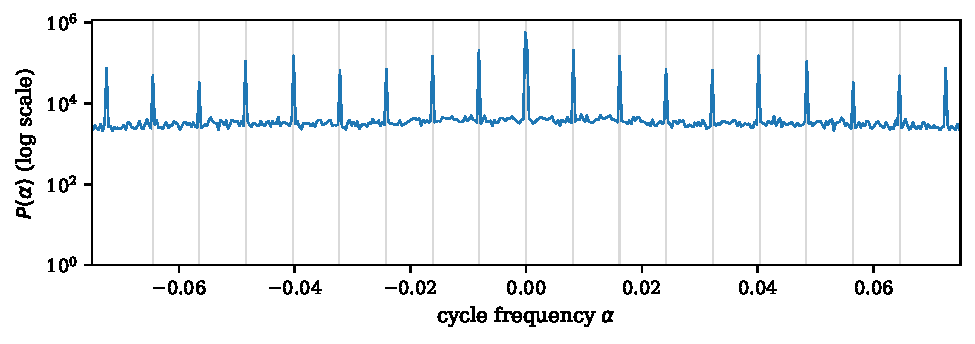
\includegraphics[width=\linewidth]{figs/fig1_sparsity.pdf}
\vspace{-6pt}
\caption{Dense alpha profile of the DSSS-BPSK test signal. Vertical grid
lines mark integer multiples of $\alpha_0$; all significant peaks
coincide with them.}
\label{fig:sparsity}
\end{figure}

\subsection{Fundamental frequency estimation}
Figure \ref{fig:scan} shows the detection statistic \eqref{eq:detstat},
computed exactly at every native bin via \eqref{eq:exact-fft} and
restricted to the search interval, together with the true $\alpha_0$. The
peak is isolated and unambiguous against the surrounding floor. Estimated
over 4096 subsampled points, $\hat\alpha_0$ matches the true fundamental to
within $0.003\%$ relative error.

\begin{figure}[t]
\centering
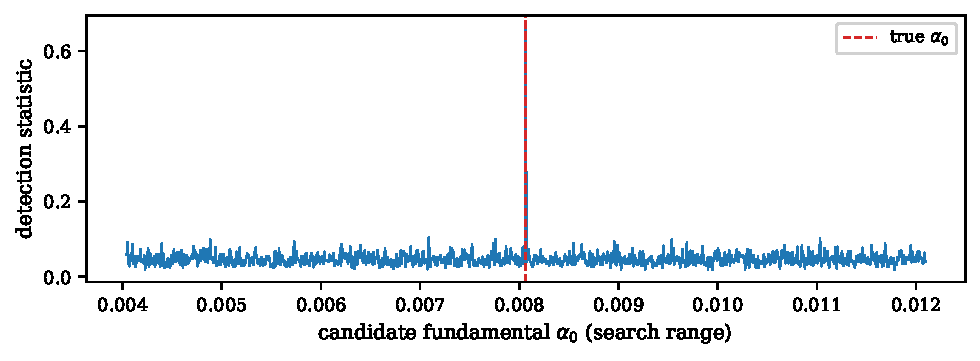
\includegraphics[width=\linewidth]{figs/fig6_scan.pdf}
\vspace{-6pt}
\caption{Detection statistic across the fundamental-frequency search
range, evaluated exactly via the zero-padded transform of
\eqref{eq:exact-fft}.}
\label{fig:scan}
\end{figure}

\subsection{Recovered profile}
Figure \ref{fig:overlay} compares the harmonic-comb estimate, obtained
from $6.25\%$ of the available samples, against the dense reference
profile on a logarithmic scale, so that strong and weak harmonics are
visible at comparable scale. The estimate lands close to the reference at
every populated cycle frequency and is silent everywhere else, consistent
with the comb model; the small offsets visible between paired markers at
a few harmonics are quantified directly in Fig.~\ref{fig:error}.

\begin{figure}[t]
\centering
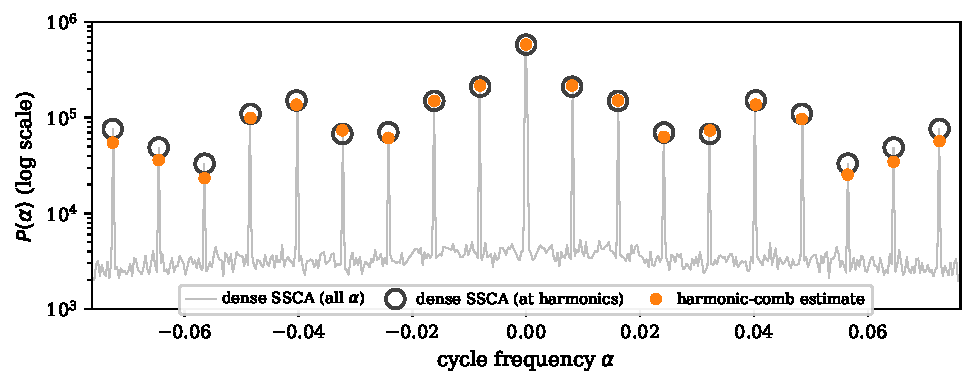
\includegraphics[width=\linewidth]{figs/fig3_overlay.pdf}
\vspace{-6pt}
\caption{Dense alpha profile compared with the harmonic-comb estimate, on
a logarithmic scale. Open circles mark the dense reference value at each
harmonic; filled circles mark the estimate at the same location, so that
agreement appears as a filled marker centered inside its open ring. The
faint background trace is the full dense profile, shown to confirm that
no comb location is missed and that the region between harmonics is
indeed silent.}
\label{fig:overlay}
\end{figure}

\subsection{Accuracy relative to reconstruction}
Figure \ref{fig:error} compares, harmonic by harmonic, the relative
magnitude error of the proposed estimator against that of full sparse SCD
reconstruction, both measured against the dense reference. Reconstruction
achieves a mean error of $2.8\%$ on populated harmonics, against roughly
$13\%$ for the comb estimator, reflecting the latter's reliance on far
fewer samples. Error is largest for the weakest, highest-order harmonics
in both methods.

\begin{figure}[t]
\centering
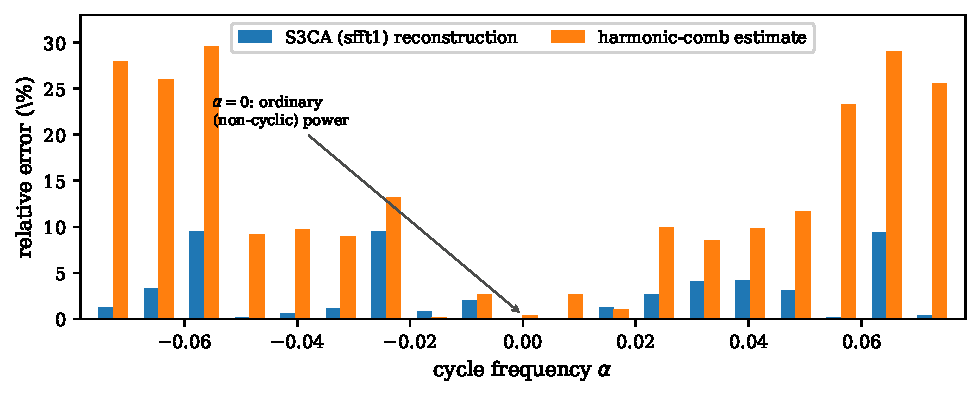
\includegraphics[width=\linewidth]{figs/fig4_error.pdf}
\vspace{-6pt}
\caption{Relative profile-magnitude error, comparing sparse SCD
reconstruction and the proposed comb estimator against the dense
reference, at each of the $2M_h+1=19$ populated cycle frequencies
$\alpha=m\alpha_0$, $m=-9,\dots,9$ (the same locations as Fig.
\ref{fig:overlay}). The bar at $\alpha=0$ reports error on the ordinary
(non-cyclic) power term rather than a harmonic proper. Positive and
negative harmonics are shown separately, since the spectral correlation
density need not be symmetric in $\alpha$, and indeed the two sides differ
appreciably (e.g.\ $\alpha=7\alpha_0$ versus $\alpha=-7\alpha_0$).}
\label{fig:error}
\end{figure}

\subsection{Computational scaling}
Figure \ref{fig:scaling} reports wall-clock time for dense reconstruction,
sparse reconstruction, and the exact-FFT comb estimator as $N$ grows from
$2^{14}$ to $2^{20}$ with the subsample count held fixed at $4096$. The
comb estimator is faster than both reconstruction methods at every $N$
tested, and its growth with $N$ is markedly gentler, consistent with
Table \ref{tab:complexity}: unlike either reconstruction method, it never
performs channelization and its cost does not scale with $N_P$.

\begin{figure}[t]
\centering
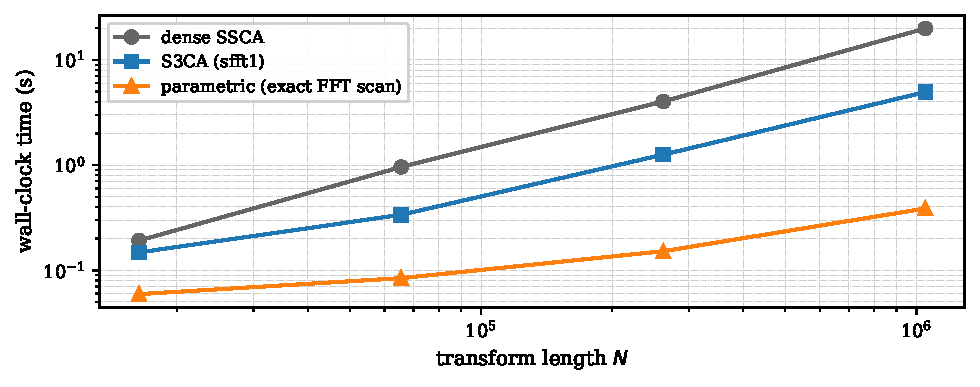
\includegraphics[width=\linewidth]{figs/fig5_scaling.pdf}
\vspace{-6pt}
\caption{Wall-clock time versus transform length $N$, fixed subsample
count.}
\label{fig:scaling}
\end{figure}

\section{Discussion}

The harmonic-comb estimator trades reconstruction accuracy for sample
economy and computational speed. Its accuracy is fundamentally limited by
the number of samples used to estimate \eqref{eq:cyclic-autocorr}, whereas
full reconstruction benefits from a complete, high-resolution transform;
the accuracy gap of roughly fourfold in Section 4.4 reflects this
difference
rather than any deficiency in the comb model itself, which was shown in
Section 4.1 to describe the profile's support exactly. The method assumes
a single fundamental cycle frequency; multiple co-channel signals, each
with its own baud rate, would require estimating and peeling one comb at a
time, analogous to successive interference cancellation. The estimator
also returns no information about the SCD away from the comb, so that
reconstruction remains necessary whenever the full surface, rather than
the profile, is required. Finally, the fundamental-frequency search
requires a search range to be supplied; a poorly chosen or excessively
wide range increases cost proportionally, since the exact-FFT evaluation
covers the full native grid but a wider range trivially admits more
false-alarm candidates for the harmonic-consistency rescoring in
\eqref{eq:combscore} to reject.

\section{Conclusion}

The alpha profile of a cyclostationary signal with a single fundamental
cycle frequency has been shown to be sparse on the harmonic comb even when
the underlying spectral correlation surface is only approximately sparse,
and a parametric estimator has been derived that exploits this structure
directly, through subsampled cyclic autocorrelation and a
harmonic-consistency rule for locating the fundamental. Recognizing that
the required non-uniform transform is exact rather than approximate, given
integer sample positions, permits its evaluation by a single zero-padded
fast Fourier transform per lag, eliminating the dependence of computational
cost on sample count and yielding an estimator that is both cheaper in
samples and faster in wall-clock time than dense or sparse reconstruction
of the full spectral correlation surface, at a moderate cost in profile
accuracy.

{\small
\begin{thebibliography}{9}

\bibitem{gardner1986}
W. A. Gardner, ``The spectral correlation theory of cyclostationary
time-series,'' \emph{Signal Processing}, vol. 11, no. 1, pp. 13--36, 1986.

\bibitem{roberts1991}
R. S. Roberts, W. A. Brown, and H. H. Loomis, ``Computationally efficient
algorithms for cyclic spectral analysis,'' \emph{IEEE Signal Processing
Magazine}, vol. 8, no. 2, pp. 38--49, 1991.

\bibitem{s3ca2015}
C. J. Li, R. Rademacher, D. Boland, C. T. Jin, C. M. Spooner, and P. H. W.
Leong, ``S$^3$CA: A sparse strip spectral correlation analyzer,'' \emph{IEEE
Signal Processing Letters}, vol. 22, no. 8, 2015.

\bibitem{hassanieh2012}
H. Hassanieh, P. Indyk, D. Katabi, and E. Price, ``Simple and practical
algorithm for sparse Fourier transform,'' in \emph{Proc. 23rd Annual
ACM-SIAM Symposium on Discrete Algorithms}, 2012, pp. 1183--1194.

\bibitem{dutt1993}
A. Dutt and V. Rokhlin, ``Fast Fourier transforms for nonequispaced
data,'' \emph{SIAM Journal on Scientific Computing}, vol. 14, no. 6, pp.
1368--1393, 1993.

\end{thebibliography}
}

\end{document}
